% Options for packages loaded elsewhere
\PassOptionsToPackage{unicode}{hyperref}
\PassOptionsToPackage{hyphens}{url}
\PassOptionsToPackage{dvipsnames,svgnames,x11names}{xcolor}
%
\documentclass[
  12pt,
]{report}

\usepackage{amsmath,amssymb}
\usepackage{setspace}
\usepackage{iftex}
\ifPDFTeX
  \usepackage[T1]{fontenc}
  \usepackage[utf8]{inputenc}
  \usepackage{textcomp} % provide euro and other symbols
\else % if luatex or xetex
  \usepackage{unicode-math}
  \defaultfontfeatures{Scale=MatchLowercase}
  \defaultfontfeatures[\rmfamily]{Ligatures=TeX,Scale=1}
\fi
\usepackage{lmodern}
\ifPDFTeX\else  
    % xetex/luatex font selection
  \setmainfont[]{Times New Roman}
  \setsansfont[]{Arial}
  \setmonofont[]{Courier New}
\fi
% Use upquote if available, for straight quotes in verbatim environments
\IfFileExists{upquote.sty}{\usepackage{upquote}}{}
\IfFileExists{microtype.sty}{% use microtype if available
  \usepackage[]{microtype}
  \UseMicrotypeSet[protrusion]{basicmath} % disable protrusion for tt fonts
}{}
\usepackage{xcolor}
\usepackage[top = 3cm,bottom = 3cm,left = 3cm,right = 2.7cm]{geometry}
\setlength{\emergencystretch}{3em} % prevent overfull lines
\setcounter{secnumdepth}{5}
% Make \paragraph and \subparagraph free-standing
\ifx\paragraph\undefined\else
  \let\oldparagraph\paragraph
  \renewcommand{\paragraph}[1]{\oldparagraph{#1}\mbox{}}
\fi
\ifx\subparagraph\undefined\else
  \let\oldsubparagraph\subparagraph
  \renewcommand{\subparagraph}[1]{\oldsubparagraph{#1}\mbox{}}
\fi


\providecommand{\tightlist}{%
  \setlength{\itemsep}{0pt}\setlength{\parskip}{0pt}}\usepackage{longtable,booktabs,array}
\usepackage{calc} % for calculating minipage widths
% Correct order of tables after \paragraph or \subparagraph
\usepackage{etoolbox}
\makeatletter
\patchcmd\longtable{\par}{\if@noskipsec\mbox{}\fi\par}{}{}
\makeatother
% Allow footnotes in longtable head/foot
\IfFileExists{footnotehyper.sty}{\usepackage{footnotehyper}}{\usepackage{footnote}}
\makesavenoteenv{longtable}
\usepackage{graphicx}
\makeatletter
\def\maxwidth{\ifdim\Gin@nat@width>\linewidth\linewidth\else\Gin@nat@width\fi}
\def\maxheight{\ifdim\Gin@nat@height>\textheight\textheight\else\Gin@nat@height\fi}
\makeatother
% Scale images if necessary, so that they will not overflow the page
% margins by default, and it is still possible to overwrite the defaults
% using explicit options in \includegraphics[width, height, ...]{}
\setkeys{Gin}{width=\maxwidth,height=\maxheight,keepaspectratio}
% Set default figure placement to htbp
\makeatletter
\def\fps@figure{htbp}
\makeatother
% definitions for citeproc citations
\NewDocumentCommand\citeproctext{}{}
\NewDocumentCommand\citeproc{mm}{%
  \begingroup\def\citeproctext{#2}\cite{#1}\endgroup}
\makeatletter
 % allow citations to break across lines
 \let\@cite@ofmt\@firstofone
 % avoid brackets around text for \cite:
 \def\@biblabel#1{}
 \def\@cite#1#2{{#1\if@tempswa , #2\fi}}
\makeatother
\newlength{\cslhangindent}
\setlength{\cslhangindent}{1.5em}
\newlength{\csllabelwidth}
\setlength{\csllabelwidth}{3em}
\newenvironment{CSLReferences}[2] % #1 hanging-indent, #2 entry-spacing
 {\begin{list}{}{%
  \setlength{\itemindent}{0pt}
  \setlength{\leftmargin}{0pt}
  \setlength{\parsep}{0pt}
  % turn on hanging indent if param 1 is 1
  \ifodd #1
   \setlength{\leftmargin}{\cslhangindent}
   \setlength{\itemindent}{-1\cslhangindent}
  \fi
  % set entry spacing
  \setlength{\itemsep}{#2\baselineskip}}}
 {\end{list}}
\usepackage{calc}
\newcommand{\CSLBlock}[1]{\hfill\break\parbox[t]{\linewidth}{\strut\ignorespaces#1\strut}}
\newcommand{\CSLLeftMargin}[1]{\parbox[t]{\csllabelwidth}{\strut#1\strut}}
\newcommand{\CSLRightInline}[1]{\parbox[t]{\linewidth - \csllabelwidth}{\strut#1\strut}}
\newcommand{\CSLIndent}[1]{\hspace{\cslhangindent}#1}

\usepackage{booktabs}
\usepackage{caption}
\usepackage{longtable}
\usepackage{colortbl}
\usepackage{array}
\usepackage{anyfontsize}
\usepackage{sectsty}
\chapterfont{\centering}
\makeatletter
\@ifpackageloaded{caption}{}{\usepackage{caption}}
\AtBeginDocument{%
\ifdefined\contentsname
  \renewcommand*\contentsname{Table of contents}
\else
  \newcommand\contentsname{Table of contents}
\fi
\ifdefined\listfigurename
  \renewcommand*\listfigurename{Figures}
\else
  \newcommand\listfigurename{Figures}
\fi
\ifdefined\listtablename
  \renewcommand*\listtablename{Tables}
\else
  \newcommand\listtablename{Tables}
\fi
\ifdefined\figurename
  \renewcommand*\figurename{Figure}
\else
  \newcommand\figurename{Figure}
\fi
\ifdefined\tablename
  \renewcommand*\tablename{Table}
\else
  \newcommand\tablename{Table}
\fi
}
\@ifpackageloaded{float}{}{\usepackage{float}}
\floatstyle{ruled}
\@ifundefined{c@chapter}{\newfloat{codelisting}{h}{lop}}{\newfloat{codelisting}{h}{lop}[chapter]}
\floatname{codelisting}{Listing}
\newcommand*\listoflistings{\listof{codelisting}{List of Listings}}
\makeatother
\makeatletter
\makeatother
\makeatletter
\@ifpackageloaded{caption}{}{\usepackage{caption}}
\@ifpackageloaded{subcaption}{}{\usepackage{subcaption}}
\makeatother
\ifLuaTeX
  \usepackage{selnolig}  % disable illegal ligatures
\fi
\usepackage{bookmark}

\IfFileExists{xurl.sty}{\usepackage{xurl}}{} % add URL line breaks if available
\urlstyle{same} % disable monospaced font for URLs
\hypersetup{
  colorlinks=true,
  linkcolor={blue},
  filecolor={Maroon},
  citecolor={Blue},
  urlcolor={blue},
  pdfcreator={LaTeX via pandoc}}

\author{}
\date{}

\begin{document}

\begin{titlepage}
  \begin{center}
    \vspace*{2cm}
    
    \Huge{\textbf{Leadership Transitions and Survival: Coups, Autocoups, and Power Dynamics}}
    
    \vspace{1.5cm}
    
    \Large{Zhu Qi}
    
    \vspace{5cm}
    
    \large{A thesis submitted for the degree of \\ Doctor of Philosophy in Political Science}
    
    \vspace{0.8cm}
    
    \large{Department of Government}
    \vspace{0.5cm}
    
    \large{University of Essex}
    
    \vspace{1.5cm}
    
    \large{September 2024}
    \vspace{2cm}
    
    \large{(Word count: 40,000 words)}
    
  \end{center}
\end{titlepage}

\renewcommand*\contentsname{Contents}
{
\hypersetup{linkcolor=}
\setcounter{tocdepth}{2}
\tableofcontents
}
\listoffigures
\listoftables
\setstretch{1.618}
\chapter*{Acknowledgements}\label{acknowledgements}
\addcontentsline{toc}{chapter}{Acknowledgements}

The completion of this thesis has been a significant journey, filled
with hard work, learning, and moments of joy. Throughout this time, I
have received support and encouragement from many individuals, without
whom this dissertation would not have been possible.

First and foremost, I would like to express my deepest gratitude to my
great supervisor, Professor Kristian Skrede Gleditsch, for his
invaluable guidance, unwavering support, and insightful feedback
throughout this journey. His expertise and encouragement have been
instrumental in shaping this dissertation. I would also like to extend
my heartfelt thanks to the chair of my board panel, Professor Han
Dorussen, for his continuous support and constructive criticism, which
have significantly enhanced the quality of my research.

I am profoundly grateful for the comments, advice, and suggestions from
several esteemed scholars who have contributed to this work. Dr.~Brian J
Phillips, Dr. Prabin Khadka, and Dr.~Winnie Xia, their expertise and
thoughtful input have been greatly appreciated and have enriched this
dissertation.

Finally, I want to thank my family for their unwavering support and
love. To my beloved wife, Ji Zhi, who has been my rock throughout this
journey, and to my dear daughter, Siyan, and son, Sisheng, who have been
my source of joy and motivation. I am deeply thankful to my father for
his enduring support, and to the memory of my late mother, whose love
and guidance continue to inspire me.

All errors and faults are my own.

\chapter*{Abstract}\label{abstract}
\addcontentsline{toc}{chapter}{Abstract}

This dissertation examines the dynamics of irregular power transitions,
particularly coups and autocoups, and their influence on leader
survival. It highlights the critical role of power dynamics, shaped by
regime types, in determining coup success rates and attempt frequency.
Utilizing Heckman's two-stage selection model, the study reveals that
expected coup success significantly influences attempts, with military
regimes facing a heightened vulnerability due to their power structure.

While often understudied, autocoups are shown to have a substantial
impact on democratic trends. This research introduces a refined
definition of autocoups alongside a novel dataset encompassing events
from 1945 to 2022, enabling a more robust quantitative analysis.

Employing survival analysis, the study compares the longevity of leaders
who rise to power through coups versus autocoups. The findings
demonstrate that coup-installed leaders face a significantly shorter
tenure and higher risk of removal. This contrasts with autocoup leaders
who manipulate the system to extend their rule, suggesting the potential
for autocoups to incentivize power grabs and contribute to democratic
backsliding.

This work contributes significantly to the political science literature
by:

\begin{itemize}
\item
  Defining key concepts: It establishes a clear definition of autocoups,
  a previously understudied phenomenon.
\item
  Introducing a novel dataset: This dataset enables researchers to
  conduct more comprehensive quantitative analyses of autocoups.
\item
  Establishing a general framework: The framework provides a comparative
  approach to studying the dynamics of irregular power transitions and
  their impact on democratic stability.
\end{itemize}

\textbf{keywords:} \emph{Coups, Autocoups, Power transitions, Leadership
Survival}

\chapter{Introduction}\label{introduction}

\section{Research question}\label{research-question}

Irregular power transitions, marked by a disregard for constitutional
procedures, are a critical area of study in political science. They not
only disrupt established rules but often require unconstitutional
tactics to secure power. Furthermore, these transitions can inspire
copycat behaviour among other ambitious leaders.

Despite their central role in political science and the extensive
research conducted on irregular power transitions, a long-standing
question continues to intrigue political scientists: \textbf{\emph{Why
are some leaders ousted before their terms expire, while others complete
their full terms or even overstay beyond their originally mandated
limits?}} In other words, why do some leaders survive for decades while
others last for only years, months, or even days? This dissertation
focuses on this question and seeks to provide a comprehensive analysis,
dedicated to understanding how leaders come to power through
unconstitutional means and what factors determine the duration of a
leader's rule following an irregular ascent.

\section{Analyses on coups and autocoups in a general
framework}\label{analyses-on-coups-and-autocoups-in-a-general-framework}

When discussing irregular power transitions, the concepts that often
come to mind are irregular entries or exits, such as coups,
assassinations, rebellions, protests, and foreign interventions. Among
these methods, coups hold a prominent position due to their frequent
occurrence. According to the Archigos dataset
(\citeproc{ref-goemans2009}{Goemans, Gleditsch, and Chiozza 2009}), from
1945 to 2015, there were approximately 145 instances of irregular leader
exits, with coups\footnote{According to the Archigos dataset, ``Removed
  by Military, without Foreign Support'' and ``Removed by Other
  Government Actors, without Foreign Support'' in the variable
  \texttt{exitcode} are classified as coups.} accounting for more than
half (79 leaders). The often-cited Global Instances of Coups
(GIC)\footnote{According to the Archigos dataset, ``Removed by Military,
  without Foreign Support'' and ``Removed by Other Government Actors,
  without Foreign Support'' in the variable \texttt{exitcode} are
  classified as coups.} dataset (\citeproc{ref-powell2011}{J. M. Powell
and Thyne 2011}) records even more leaders (245 cases) removed by coups
from 1950 to 2023.

Given their prevalence and substantial influence on political systems,
coups have been extensively studied, particularly since 2000
(\citeproc{ref-thyne2019}{Thyne and Powell 2019}). Consequently, the
concept of a coup is comparatively clear and widely accepted in academic
circles. Many scholars, including this study, follow the definition by
J. M. Powell and Thyne (\citeproc{ref-powell2011}{2011}), which
describes coups as ``illegal and overt attempts by the military or other
elites within the state apparatus to unseat the sitting
executive\ldots{} {[}a coup is successful{]} if the perpetrators seize
and hold power for at least seven days'' (p.~252). Although debates
persist, two elements are clear: first, the perpetrators are elites
within the ruling group, and the victims of coups are incumbent
executive leaders. Second, the strategy or aim of a coup involves
completely removing the incumbents, not merely seizing part of their
power or forcing them to concede on specific policies. Beyond defining
coups, several datasets have been developed for quantitative analyses,
such as the Global Instances of Coups (\citeproc{ref-powell2011}{J. M.
Powell and Thyne 2011}), the Cline Centre Coup d'État Project Dataset
(\citeproc{ref-peyton2024}{Peyton et al. 2024}), and the Colpus Dataset
(\citeproc{ref-chin2021}{Chin, Carter, and Wright 2021}). These datasets
are well-developed and frequently used in political science research.

However, irregular power transitions are not limited to irregular
entries and exits but should also include irregular ``overstays.'' Using
illegal means to overthrow an incumbent leader before their term expires
is undoubtedly an irregular power transition. Similarly, an incumbent
using illegitimate means to extend their term beyond term limits is also
an irregular power transition.

Although academic attention to irregular retention of power has
increased since the 1990s, especially after Peru's President Alberto
Fujimori's self-coup in 1992, it remains comparatively understudied and
has several shortcomings. First, there is no universally accepted
terminology for this ``overstaying in power'' type of irregular power
transition, unlike the clear term ``coup.'' Consequently, various terms
such as self-coup, autogolpe, and executive coup are used by different
scholars. This dissertation will use `autocoup' to refer to this type of
irregular power transition, which will be thoroughly discussed in
Chapter 3. Second, there is no consensus on the definition of an
autocoup. Existing definitions remain vague, often conflating power
expansions and power extensions\footnote{The definitions and concepts of
  power expansion and power extension can be vague. In this study, we
  define power expansion as an incumbent acquiring additional authority
  from other state apparatuses, whereas power extension refers to an
  incumbent prolonging their tenure beyond the designated term in
  office.}. For example, Cameron (\citeproc{ref-cameron1998a}{1998})
defines an autogolpe as a temporary suspension of the constitution and
dissolution of Congress by the executive, who then rules by decree. This
definition focuses on power expansion instead of power extension,
leading to conceptual confusion and misalignment with the definition of
a classic coup. Third, a consensus autocoup dataset is lacking. While
several related datasets exist, as discussed by Baturo and Tolstrup
(\citeproc{ref-baturo2022}{2022}) in coding their Incumbent Takeover
dataset, the terminologies, definitions, and coverage years vary,
lacking wide acknowledgement and extensive academic exploration. In
summary, autocoup has not been analysed in a comparative manner
connected with coups.

Analysing coups and autocoups separately is less problematic. However,
from a comprehensive framework perspective on irregular power
transitions and leader survival, coups and autocoups should be, and can
be, analysed within the same framework. Both coup and autocoup
significantly influence democratic backsliding and are the most frequent
means of irregular power transition. Furthermore, as both are called
``coups,'' classic coups and autocoups are very similar since a coup is
launched to replace the current leader, while an autocoup is staged to
replace the future leader.

\section{Academic Contributions}\label{academic-contributions}

This study addresses a critical gap in the literature by offering a
comprehensive framework for analysing both coups and autocoups, which
are the most common forms of irregular power transitions. While existing
research often examines these topics separately with varying
terminologies, definitions, methods, and datasets, this dissertation
integrates these elements to provide a unified perspective on irregular
power transitions and leader survival.

Our contributions are threefold:

\begin{itemize}
\item
  \textbf{Emphasis on power dynamics and regime types}: We highlight the
  significant role of power dynamics, particularly the influence of
  regime types, in determining the success and frequency of coup
  attempts. Our analysis underscores how the expected chances of coup
  success motivate such attempts, with military regimes being notably
  susceptible.
\item
  \textbf{Refined definition and novel dataset for autocoups:} We
  introduce a refined definition of autocoups and develop a novel
  dataset covering events from 1945 to 2022. This enables a comparative
  analysis with classic coups, providing clearer insights into the
  nature and impact of autocoups on political systems.
\item
  \textbf{Survival analysis of leaders from different entry modes:} By
  applying survival analysis to existing coup data and our new autocoup
  dataset, we demonstrate how different modes of entry into power
  significantly affect leader survival. Our findings reveal that leaders
  who come to power through coups typically have shorter tenures and
  face higher removal risks compared to those who extend their rule
  through autocoups.
\end{itemize}

Our analysis of irregular power transitions is particularly relevant to
understanding democratic backsliding. These transitions violate
democratic norms and disrupt the path towards stable democracy. Leaders
who gain power through irregular means often employ undemocratic
tactics, such as suppressing opposition, to consolidate their
illegitimate hold on power. This creates a vicious cycle where the
erosion of democratic institutions is both a cause and consequence of
efforts to maintain power.

\section{Overview of the thesis}\label{overview-of-the-thesis}

This study is structured into three main chapters beyond the
introduction, each addressing key aspects of irregular power transitions
and their implications for political stability and democratic processes.

\textbf{Chapter 2} examines the determinants of classic coup attempts.
While extensive research exists on coups, most studies focus on
observable factors such as economic performance, political stability,
previous coups, and coup-proofing strategies. This chapter, however,
emphasizes the less observable but crucial factor of expected coup
success chances, which has been often overlooked. Utilizing Heckman's
two-staged sample selection model, the analysis reveals that expected
success rates significantly influence coup attempts. These success rates
are primarily shaped by the balance of power between incumbents and
challengers, which is largely determined by regime types. The findings
indicate that military regimes face a much higher risk of coups compared
to dominant-party regimes.

\textbf{Chapter 3} focuses on the concept of autocoups, specifically on
power extensions by incumbent leaders. It distinguishes autocoups from
broader concepts like self-coups or executive coups by redefining them
as instances where incumbent leaders refuse to transition power as
mandated, thereby overstaying in office. Based on this refined
definition, a novel dataset of autocoup events from 1945 to 2022 is
introduced, encompassing 110 attempts and 87 successes. The chapter
includes case studies and empirical analyses that demonstrate the
utility of this dataset for quantitative research, providing a basis for
empirical analysis on autocoups.

\textbf{Chapter 4} investigates how the method of power acquisition
impacts the longevity of leaders who come to power through coups versus
those who extend their rule through autocoups. The hypothesis is that
the method of accession significantly affects leader tenure. Using the
Cox proportional hazards model and a time-dependent Cox model, the
chapter provides evidence of differing survival times between these two
types of leaders. The results indicate that leaders who come to power
through coups face a significantly higher risk of removal compared to
those who extend their rule through autocoups. This finding highlights
the implications for political stability and democratic processes,
suggesting that the relatively low cost and high returns of autocoups
could incentivize incumbents to seize power in this manner, potentially
leading to democratic backsliding and the personalization of power.

In \textbf{Chapter 5}, the study concludes by summarizing the main
findings, discussing policy implications, and acknowledging the
limitations of the research. It also outlines directions for future
research, emphasizing the need for further exploration of irregular
power transitions, particularly coups and autocoups.

\chapter{Power Dynamics and Coup Attempts: A Selection Mechanism
Analysis}\label{power-dynamics-and-coup-attempts-a-selection-mechanism-analysis}

\section{Introduction}\label{introduction-1}

Coups occur with varying frequency across different countries, with some
experiencing them more frequently than others. According to GIC dataset,
Latin American countries such as Bolivia witnessed 23 coups between
\(1950\) and \(1984\), while Argentina experienced 20 during a similar
time frame. However, Mexico's authoritarian period from \(1917\) to
\(2000\) saw no coups at all. In Africa, Sudan endured 17 coups between
\(1955\) and \(2023\), whereas South Africa has not experienced any coup
since \(1950\). Similar patterns are observed in the Middle East and
South Asia.

The varying frequency of coup attempts has captivated political
scientists for decades, leading to extensive research on the subject. As
highlighted by Gassebner, Gutmann, and Voigt
(\citeproc{ref-gassebner2016}{2016}), despite approximately one hundred
potential determinants of coups being suggested, no consensus has been
reached. In an effort to address this issue, Gassebner, Gutmann, and
Voigt (\citeproc{ref-gassebner2016}{2016}) tested 66 factors proposed in
previous literature using three million model permutations in an extreme
bounds analysis.

Examining previous research, which has tested around 100 variables as
potential determinants of coups, raises an important question beyond
simply understanding why coups are more frequent in some countries than
others. The critical question is: Can we establish a method to help
scholars focus on the most relevant factors of coups, rather than
sifting through over 100 variables without reaching a consensus?

Reviewing previously proposed variables of coups, it is evident that all
focus on pre-coup conditions, with no consideration given to post-coup
factors. However, coups are high-stakes gambles with an all-or-nothing
nature. As defined by J. M. Powell and Thyne
(\citeproc{ref-powell2011}{2011}), coups are ``illegal and overt
attempts by the military or other elites within the state apparatus to
unseat the sitting executive'' (\citeproc{ref-powell2011}{J. M. Powell
and Thyne 2011, 252}). Due to their illegality, the consequences of a
failed coup can be severe, with perpetrators risking imprisonment,
exile, or even death. In some instances, repercussions extend to the
families of the coup perpetrators. Therefore, no coup plotters would
stage a coup without some assurance of success.

Historical coup attempts and their success rates provide valuable
insights. Despite the significant risks associated with coups since
1950, as shown in Table~\ref{tbl-coups}, there have been 491 coups
worldwide. Importantly, about half of these coups have been successful.
At first glance, coups appear to be a high-success-rate political
venture. However, compared to over 12,000 country-years since 1950, the
occurrence of 491 coups is relatively rare, accounting for about 4\%
(\citeproc{ref-powell2011}{J. M. Powell and Thyne 2011}).

The low occurrence rate and high success rate clearly indicate that the
initiation of coups is highly selective. In other words, the likelihood
of a coup occurring depends greatly on its potential success rate. Since
coup plotters meticulously assess potential outcomes, we should also
analyze what factors most affect these outcomes when discussing the key
determinants of coups. This approach allows us to focus on the most
relevant factors and disregard those less related.

\begingroup
\setlength\LTleft{0.05\linewidth}
\setlength\LTright{0.05\linewidth}\fontsize{12.0pt}{14.4pt}\selectfont
\setlength{\LTpost}{0mm}

\begin{longtable}{@{\extracolsep{\fill}}lccr}

\caption{\label{tbl-coups}Top 10 countries with the most coup attempts}

\tabularnewline

\toprule
Country & Coup Attempted & Coup Succeeded & Success Rate \\ 
\midrule\addlinespace[2.5pt]
Bolivia & 23 & 11 & 47.8\% \\ 
Argentina & 20 & 7 & 35.0\% \\ 
Sudan & 17 & 6 & 35.3\% \\ 
Haiti & 13 & 9 & 69.2\% \\ 
Venezuela & 13 & 0 & 0.0\% \\ 
Iraq & 12 & 4 & 33.3\% \\ 
Syria & 12 & 8 & 66.7\% \\ 
Thailand & 12 & 8 & 66.7\% \\ 
Ecuador & 11 & 5 & 45.5\% \\ 
Burundi & 11 & 5 & 45.5\% \\ 
Guatemala & 10 & 5 & 50.0\% \\ 
Total & 491 & 245 & 49.9\% \\ 
\bottomrule

\end{longtable}

\begin{minipage}{\linewidth}
\emph{Source: GIC dataset}\\
\end{minipage}
\endgroup

When considering the factors that most affect the outcomes of coups, the
current literature predominantly identifies military power as the
decisive factor in the success of coups. This necessitates an analysis
of power dynamics within regimes, as military power is ultimately shaped
by power dynamics.

Because coup attempts are self-selective rather than random, this study
employs a double \texttt{probit} model with sample selection to examine
factors influencing coup success rates and, consequently, the likelihood
of coup attempts. I posit that regime type, by shaping internal power
dynamics among coup plotters, incumbents, and other ruling elites, is a
crucial determinant of coup likelihood.

This study makes two key contributions to the existing literature.
First, it underscores the importance of regime type as a crucial
determinant of coup attempts. Previous studies often treat regime type
as a control variable, overlooking that variations in many other
variables are fundamentally rooted in different regime types. More
importantly, this study establishes a systematic approach for
identifying the most relevant factors, thereby avoiding sifting through
over 100 variables.

The subsequent section explores the dynamics of coup attempts and their
outcomes. In section 3, I detail the research design, outlining the
methodology and variables used in the analysis. Section 4 presents and
discusses the empirical findings. Section 5 concludes this chapter,
summarizing the key insights and their implications.

\section{Dynamics of coup attempts and
outcomes}\label{dynamics-of-coup-attempts-and-outcomes}

Coup attempts are driven by a complex interplay of factors, with two key
elements attracting significant scholarly attention:
\textbf{disposition} (the motivations behind the attempt) and
\textbf{capability} (the resources and opportunities to succeed).

\subsection{Motivations for coups}\label{motivations-for-coups}

This section focuses on disposition, exploring the primary motivations
that compel individuals to undertake the significant risks associated
with a coup. We can categorize coup motivations into three main types:

\textbf{Personal Ambition:} The allure of absolute power, prestige, and
wealth is a significant motivator for some coup plotters. For example,
Wintrobe (\citeproc{ref-wintrobe2019}{2019}) distinguishes between
totalitarian and tinpot dictators based on their use of power. While
both prioritize personal gain, totalitarian leaders seek complete
control over every aspect of society, whereas tinpot leaders focus on
enriching themselves through extravagant lifestyles.

\textbf{Purported National Interest:} Coups are sometimes justified as
necessary interventions to save a nation from crisis, uphold the
constitution, or facilitate a transition to democracy. While scepticism
is warranted due to the potential for self-serving justifications,
legitimate cases do exist. For instance, the 2010 coup in Niger ousted
President Tandja, who attempted an unconstitutional third term by
dissolving the opposing court and calling a self-serving referendum
(\citeproc{ref-ginsburg2019}{Ginsburg and Elkins 2019}).

\textbf{Self-Preservation:} In some instances, coups are pre-emptive
strikes against imminent political persecution or repression. Coup
leaders might not be motivated by a desire for power, but rather a fear
of elimination by the incumbent regime. A notable example is Idi Amin's
1971 coup against Ugandan President Obote, who was attempting to remove
Amin from his military command position
(\citeproc{ref-sudduth2017}{Sudduth 2017}).

These motivations can arise in any regime, but autocracies are
particularly susceptible, especially for coups framed under the guise of
national interest or self-preservation. Stable democracies, on the other
hand, rarely face the same level of constitutional crises or political
persecution that might necessitate a coup. However, new democracies can
be vulnerable to instability, economic downturns, and democratic
backsliding, creating opportunities for coup plotters to exploit these
weaknesses and justify their actions.

Despite the potential motivations outlined above, coups remain
relatively uncommon events, occurring in only about 4\% of country-years
since 1950. This low frequency highlights the importance of the second
key element -- capability. Even the most motivated plotters require the
resources and opportunities to succeed. No rational actor attempts a
guaranteed failure; the next section will explore the concept of
capability in greater detail.

\subsection{Capability for coups}\label{capability-for-coups}

While many ambitious individuals may covet supreme power, only a select
few possess the capability to orchestrate a successful coup. This
capability hinges not just on their desire, but on overcoming inherent
disadvantages compared to the incumbent leaders.

Firstly, coups are inherently clandestine operations due to their
illegality. Plotters require a tight-knit group to minimize leaks and
maximize the element of surprise. This secrecy restricts their ability
to openly recruit supporters, a privilege enjoyed by incumbents who can
implement ``coup-proofing'' measures.

Secondly, coup plotters face uncertainty about the reactions of other
powerful factions within the regime, those who could tip the scales of
power. Incumbents, however, have a deeper understanding of these
dynamics and proactively work to solidify their own position. While they
may not know who exactly might attempt a coup, they are attuned to
potential threats and adapt their strategies accordingly.

Thirdly, coup plotters face a significant challenge in securing
unwavering loyalty from potential co-conspirators. The risks associated
with a coup are substantial, with uncertain rewards even in the event of
success. Promises made by coup leaders might not be kept, and post-coup
purges are a common tactic to eliminate future coup threats. Defecting
to the incumbent leader can often be a safer option, offering
predictable rewards and less risk.

Given these inherent obstacles, rational coup plotters are unlikely to
gamble on a low-probability attempt. They may choose to abandon their
plans altogether or bide their time for a more opportune timing.
Therefore, when coup plotters do take action, it is because they have
meticulously assessed their chances of success and believe the risks are
outweighed by the potential gains.

But what is the threshold for a ``good enough'' chance of success?
Before diving into a theoretical framework, let's examine historical
data to gain some perspective. Surprisingly, coups since 1950 boast a
rather high success rate, with nearly half ending in victory (as shown
in Table~\ref{tbl-coups}).

\subsection{Framework of coup success}\label{framework-of-coup-success}

An oft-cited framework (\citeproc{ref-gassebner2016}{Gassebner, Gutmann,
and Voigt 2016}; \citeproc{ref-aidt2019}{Aidt and Leon 2019}) provides a
structured approach to assess the disposition and capability of coup
attempts by evaluating the anticipated benefits for coup plotters. The
expected payoff of coups can be represented by the equation:

\begin{equation}\phantomsection\label{eq-eq1}{
\begin{aligned}
E(U) = p \times B + (1 - p) \times (-C)
\end{aligned}
}\end{equation}

Here, \(\mathbf B\) represents the return of a successful coup,
\(\mathbf C\) signifies the cost of a failed coup, and \(p\) represents
the probability of coup success. The condition for staging a coup is
when the expected benefit is positive, meaning that the expected pay-off
is greater than 0. Rearranging the equation, we get:

\begin{equation}\phantomsection\label{eq-eq2}{
\begin{aligned}
p \times B > (1 - p) \times C
\end{aligned}
}\end{equation}

Equation~\ref{eq-eq2} implies that for Equation~\ref{eq-eq1} to hold,
the expected benefits earned from successful coups must outweigh the
expected cost of failed coups.

While seemingly clear, the equation faces practical challenges.
Quantifying \(\mathbf B\) (the value of a successful coup) and
\(\mathbf C\) (the cost of failure) is difficult. The loss of life,
freedom, or loved ones after a failed coup, as well as the value of
assuming leadership after a successful coup, are intangible concepts
that defy precise measurement. As evidenced by the 1979 coup in
Ghana\footnote{According to the Archigos dataset, ``Removed by Military,
  without Foreign Support'' and ``Removed by Other Government Actors,
  without Foreign Support'' in the variable \texttt{exitcode} are
  classified as coups.}, the fate of the coup leader(s) hangs in the
balance; they are high likely to be killed if the coup fails, or to
execute others if the coup succeeds.

However, these challenges do not render the framework useless. Firstly,
its core logic remains valuable, offering insights into how coup
plotters might assess the return and cost of their actions. Secondly,
given the significant and elusive nature of precise values for
\(\mathbf B\) and \(\mathbf C\), they can be treated as roughly equal.
Consequently, there is no need to fret over how to measure and compare
these values precisely. Instead, we can shift our focus from
\(\mathbf B\) and \(\mathbf C\), to the probability of success (\(p\)),
simplifying Equation~\ref{eq-eq2} to:

\begin{equation}\phantomsection\label{eq-eq3}{
\begin{aligned}
p > (1-p)
\end{aligned}
}\end{equation}

Equation~\ref{eq-eq3} suggests that, to hold Equation~\ref{eq-eq2} true,
a success probability greater than \(50\%\) is necessary. Interestingly,
empirical data on coups since 1950 somewhat supports this notion. As
shown in Table~\ref{tbl-coups}, the overall success rate is \(49.9\%\).
While this falls short of the \(50\%\) threshold, it's important to
consider two factors. Firstly, this is an average rate, not necessarily
reflective of the probabilities assessed by coup plotters beforehand.
Secondly, outliers such as irrational actors and coups driven by
self-preservation may not prioritize success probabilities. Taking these
points into account, we can propose our first hypothesis:

\begin{quote}
\textbf{\emph{H1: The fundamental determinant of a coup attempt is the
perceived chance of success. Coup plotters likely require a success
threshold of at least 50\%.}}
\end{quote}

This leads us to the next crucial question: what factors determine a
coup's success, influencing the very decision to attempt one? While
specifics may vary, the core element hinges on the power dynamic between
coup plotters and the incumbent leaders. Logically, the more powerful
entity holds a greater advantage in this high-stakes struggle for
control.

\subsection{Regime types and power
dynamics}\label{regime-types-and-power-dynamics}

Military strength undeniably plays a critical role in coup attempts.
Control of the armed forces offers a significant advantage, explaining
why military coups dominate discussions on the topic. Much of the
literature treats ``coup'' and ``military coup'' interchangeably, with
scholars like J. M. Powell and Thyne (\citeproc{ref-powell2011}{2011})
finding half of 14 studies attribute coups solely to the military.
Consequently, significant focus, from both researchers and policymakers,
centers on the balance of power between civilian and military
authorities, or among military factions themselves. Strategies like
``keeping the military content'' (\citeproc{ref-aidt2019}{Aidt and Leon
2019}) or ``providing them with resources''
(\citeproc{ref-huntington1991democratization}{Huntington 1991}) aim to
reduce military intervention. Empirical research informs coup-proofing
strategies that either decrease the military's desire for coups or raise
barriers to success (\citeproc{ref-leon2013a}{Leon 2013};
\citeproc{ref-powell2018}{J. Powell et al. 2018}).

However, while military power is decisive, previous literature often
oversimplifies its nature. As Table~\ref{tbl-regimes} will demonstrate,
military regimes, despite concentrated military control, exhibit
surprising instability. Military regimes experience most frequent coup
attempts. This highlights a crucial oversight: the intra-military
component. Treating the military as a monolithic entity ignores the
complex internal dynamics (\citeproc{ref-singh2016}{Singh 2016}).
Regardless of size, any military comprises diverse groups with their own
hierarchies, fostering suspicion, competition, and vigilance rather than
unity. The clandestine nature of coups necessitates small, secretive
groups. Plotters are unsure of other factions' stances and fear their
opposition or intervention, as exemplified by the swiftly thwarted 2021
Niger coup\footnote{The definitions and concepts of power expansion and
  power extension can be vague. In this study, we define power expansion
  as an incumbent acquiring additional authority from other state
  apparatuses, whereas power extension refers to an incumbent prolonging
  their tenure beyond the designated term in office.}. The success of a
coup hinges heavily on other military factions' reactions
(\citeproc{ref-geddes1999}{Geddes 1999}).

Furthermore, the relationship between government and military varies
across regimes. In democracies, civilian authority reigns supreme. The
military is a national institution bound by the constitution, not
individual leaders, ensuring political neutrality (e.g., the U.S. Armed
Forces). Conversely, non-democracies display a less clear power
structure. Identifying the true leader of the military depends on the
regime type. We will leverage framework of Geddes, Wright, and Frantz
(\citeproc{ref-geddes2014}{2014}) to categorize autocracies based on
leadership origin and decision-making. This framework classifies regimes
into three main categories: military, personalist, and dominant-party.

\textbf{Military regimes} are characterized by the dominance of a junta
-- a group of military officers who control the regime's power
structure, including leadership selection and policy formulation.
Examples include the Brazilian regime (1964-1985), the Argentine regime
(1976-1983), and the Salvadoran regime (1948-1984)
(\citeproc{ref-geddes1999}{Geddes 1999}). In \textbf{personalist
regimes}, power resides with a single, charismatic leader who controls
policy, the military, and succession. Regimes like Rafael Trujillo's in
the Dominican Republic (1930-1961), Idi Amin's in Uganda (1971-1979),
and Jean-Bédel Bokassa's in the Central African Republic (1966-1979)
exemplify personalist rule (\citeproc{ref-geddes1999}{Geddes 1999}). In
\textbf{dominant-party regimes,} power rests within a well-organized
ruling party, with leaders acting as its representatives. The party
structure and ideology foster internal cohesion and a long-term vision.
Examples include the Partido Revolucionario Institucional (PRI) in
Mexico, the Revolutionary Party of Tanzania (CCM), and Leninist parties
in various Eastern European countries (\citeproc{ref-geddes1999}{Geddes
1999}).

The critical distinction between regime types lies in the unique power
balance established during the initial power seizure. The most competent
group, be it a military junta, a political party, or a strongman,
typically prevails due to the challenges of seizing control. This power
grab is often accompanied by purges of potential rivals, solidifying the
newly established regime (\citeproc{ref-sudduth2017}{Sudduth 2017};
\citeproc{ref-roessler2011}{Roessler 2011}).

Following these internal purges and external challenges, a new power
dynamic emerges, typically solidifying into one of three main
structures: military regimes, personalist regimes, or dominant-party
regimes.

\begin{itemize}
\item
  \textbf{Dominant-Party Regimes:} These regimes boast the greatest
  stability due to their institutionalized structure. A dominant party,
  with its shared ideology and goals, fosters internal cohesion and a
  long-term vision. Power resides within the party, not with any single
  individual, and the military aligns with the party itself,
  contributing to greater stability. Formalized succession rules further
  bolster stability by ensuring a smooth transfer of power
  (\citeproc{ref-frantz2016}{Frantz and Stein 2016}).
\item
  \textbf{Personalist Regimes:} These regimes exhibit a degree of
  initial stability as dictators, having emerged from intense
  competition, are typically tough and competent. The purging of rivals
  creates a temporary status quo within the dictator's inner circle.
  However, the lack of a clear succession plan creates a vulnerability.
  The dictator's sudden death can plunge the regime into chaos, as
  potential successors scramble for power, creating a prime opportunity
  for coups.
\item
  \textbf{Military Regimes:} These regimes are often the least stable.
  Power is typically shared among a junta, leading to mistrust and
  internal conflicts over benefits and policies. The absence of a single
  authority figure hinders decisive action, as exemplified by the power
  struggles within the Chilean junta after the 1973 coup
  (\citeproc{ref-arriagadaherrera1988}{Arriagada Herrera 1988}).
\end{itemize}

\begingroup
\setlength\LTleft{0\linewidth}
\setlength\LTright{0\linewidth}\fontsize{12.0pt}{14.4pt}\selectfont
\setlength{\LTpost}{0mm}

\begin{longtable}{@{\extracolsep{\fill}}>{\raggedright\arraybackslash}p{22.5pt}>{\raggedright\arraybackslash}p{22.5pt}>{\raggedleft\arraybackslash}p{60pt}>{\raggedright\arraybackslash}p{135pt}}

\caption{\label{tbl-regimes1}Main features of different types of
regimes}

\tabularnewline

\toprule
Regime Type & Center of Power & Institutionalized Leadership Succession & Power Transition \\ 
\midrule\addlinespace[2.5pt]
Military  & Junta & 59\% & Based on agreement among
junta members \\ 
Personalist & Dictator & 77\% & Dependent on dictator’s
health or lifepan \\ 
Dominant-party & Party & 97\% & Structured by the party’s
institutional frameworks \\ 
\bottomrule

\end{longtable}

\begin{minipage}{\linewidth}
\emph{Source: GWF \& Author}\\
\end{minipage}
\endgroup

These contrasting power dynamics significantly influence a regime's
susceptibility to coups. As Table~\ref{tbl-regimes} confirms, military
regimes, despite representing only 5.6\% of country-years, experience a
disproportionate share of coups (over 22\%). Personalist regimes follow
a similar pattern, facing a higher coup risk (23\% of coups) despite
constituting only 13\% of country-years. Conversely, dominant-party
regimes, with their institutionalized structures and unified leadership,
exhibit the greatest resilience. They represent 22.6\% of country-years
but experience a lower incidence of coups (only 16.7\%).

\begingroup
\setlength\LTleft{0\linewidth}
\setlength\LTright{0\linewidth}\fontsize{12.0pt}{14.4pt}\selectfont
\setlength{\LTpost}{0mm}

\begin{longtable}{@{\extracolsep{\fill}}lrrrrr}

\caption{\label{tbl-regimes}Regime types and coups since 1950}

\tabularnewline

\toprule
Regime Type & Country Year & Share & Num of Coups & Percent of Coups & Success Rate \\ 
\midrule\addlinespace[2.5pt]
Democracy & 5303 & 46.7\% & 122 & 24.8\% & 51.6\% \\ 
Dominant-Party & 2569 & 22.6\% & 82 & 16.7\% & 53.7\% \\ 
Personal & 1477 & 13.0\% & 113 & 23.0\% & 44.2\% \\ 
Monarchy & 1056 & 9.3\% & 25 & 5.1\% & 56.0\% \\ 
Military & 638 & 5.6\% & 110 & 22.4\% & 48.2\% \\ 
Other & 322 & 2.8\% & 39 & 7.9\% & 53.8\% \\ 
Total & 11365 & 100.0\% & 491 & 100.0\% & 49.9\% \\ 
\bottomrule

\end{longtable}

\begin{minipage}{\linewidth}
\emph{Source: REIGN and GIC Datasets}\\
\end{minipage}
\endgroup

\begin{quote}
\textbf{\emph{H2: Due to their balance of power dynamics, military
regimes are more prone to coups, followed by personalist regimes, while
dominant-party regimes are the least likely to experience coups among
the three.}}
\end{quote}

\section{Research Design}\label{research-design}

\subsection{Double probit with sample selection
model}\label{double-probit-with-sample-selection-model}

This study employs a sophisticated statistical approach to account for
the selective nature of coup attempts. While coup attempt rates vary
across regimes (as discussed previously), success rates tend to be
surprisingly consistent, hovering around 50\% (as shown in
Table~\ref{tbl-regimes}). This suggests that coup attempts are not
random acts, but rather strategically planned and undertaken only when
the odds of success appear favourable. A standard statistical model
would not account for this selectivity, potentially leading to biased
results.

To address this issue, we utilize a two-stage sample selection model,
similar to the approach used by J. Powell
(\citeproc{ref-powell2012}{2012}). This model has two parts:

\begin{itemize}
\item
  \textbf{Selection Equation (Stage 1):} This stage analyzes the factors
  influencing whether a coup attempt occurs in a particular regime. The
  primary explanatory variable here is regime type, as previously
  discussed. Additional control variables may also be included, denoted
  by \(\mathbf{XB}\).
\item
  \textbf{Outcome Equation (Stage 2):} This stage focuses on the
  probability of success for those coup attempts that actually take
  place.
\end{itemize}

The primary explanatory variables are regime types, as previously
discussed. Control variables are included in \(\mathbf{XB}\). The
selection equation (first stage) models the probability that a coup
attempt occurs and can be expressed as follows:

\begin{equation}\phantomsection\label{eq-eq4}{
\begin{aligned}
y_1^*=\alpha_0 + \alpha_1 Regime_i + \mathbf {XA} + \mu_{1i}
\end{aligned}
}\end{equation}

Here, \({y_1}^*\) is an unobserved variable, which may be known to coup
plotters. \(Regime_i\) is a categorical variable (\emph{military},
\emph{personalist}, or \emph{dominant-party}). \(\mathbf{XB}\) captures
other control variables, such as the economic crisis index, previous
coups, military expenditure, etc.

The observed binary outcome \(\mathbf{y_1}\) is:

\[
\begin{aligned}
y_1 = 
\begin{cases} 
1 &\text{if $y_1^*>0$ (coup attempt occurs)} \\
0 &\text{if $y_1^*\le0$ (no coup attempt)}
\end{cases}
\end{aligned}
\]\\
In the first stage, if \(y_1^*\le0\), no coup attempt occurs in a given
country-year, indicating that the unobserved variable does not reach the
threshold. If \(y_1^*>0\), at least one coup attempt is made in a
country-year, indicating that the unobserved variable surpasses the
threshold. The probability is expressed as:

\begin{equation}\phantomsection\label{eq-eq4a}{
\begin{aligned}
Prob(y_1 =1)&=Prob(y_{1}^*>0) \\
&=\Phi(\alpha_0 + \alpha_1 Regime_i + \mathbf{XA})
\end{aligned}
}\end{equation}

Similarly, the outcome equation (second stage) models the probability
that a coup attempt is successful, given that it occurs:

\begin{equation}\phantomsection\label{eq-eq5}{
\begin{aligned}
y_2^*=\beta_0 + \beta_1 Regime_i + \mathbf {XB} + \mu_{2i}
\end{aligned}
}\end{equation}

The observed outcome \(y_2\) is:

\[
\begin{aligned}
y_2 = 
\begin{cases} 
1 &\text{if $y_2^*>0$ (coup succeeds)} \\
0 &\text{if $y_2^*\le0$ (coup fails)}
\end{cases}
\end{aligned}
\]

The probability equations is:

\begin{equation}\phantomsection\label{eq-eq5a}{
\begin{aligned}
Prob(y_2=1|y_1 =1)=\Phi(\beta_0 + \beta_1 Regime_i + \mathbf{XB})
\end{aligned}
}\end{equation}

\subsection{Variables}\label{variables}

\begin{itemize}
\tightlist
\item
  Dependent variable
\end{itemize}

Our analysis utilizes data on coup attempts and outcomes from J. M.
Powell and Thyne (\citeproc{ref-powell2011}{2011}). A successful coup is
defined as one where the incumbent leader is removed from power for more
than seven days. The dataset covers the period from 1950 to 2023 and
includes information on 491 coup attempts, with roughly half (245) being
successful. Descriptive statistics for these coup attempts and regime
types can be found in Table~\ref{tbl-coups} and Table~\ref{tbl-regimes}.

\begin{itemize}
\tightlist
\item
  Key Independent Variable: Regime Type
\end{itemize}

The core variable of interest is regime type, categorized following the
classification system of Geddes, Wright, and Frantz
(\citeproc{ref-geddes2014}{2014}) (GWF). We focus on military,
personalist, and dominant-party regimes, with democracies and monarchies
included for comparison. Descriptive statistics for regime types are
presented in Table~\ref{tbl-regimes}.

\begin{itemize}
\tightlist
\item
  Control variables
\end{itemize}

Our control variables are chosen based on the research of Gassebner,
Gutmann, and Voigt (\citeproc{ref-gassebner2016}{2016}). They analyzed
66 factors potentially influencing coups and found that slow economic
growth, prior coup attempts, and other forms of political violence are
particularly significant factors. Therefore, we include economic
performance, political violence, and the number of previous coups as our
main control variables.

\textbf{Economic Performance:} We measure economic performance using the
current-trend (\(CT\)) ratio developed by Krishnarajan
(\citeproc{ref-krishnarajan2019}{2019}). This ratio compares a country's
current GDP per capita to the average GDP per capita over the previous
five years. A higher \(CT\) ratio indicates stronger economic
performance. We use GDP per capita data (in constant 2017 international
dollars, PPP) from the V-Dem dataset by Fariss et al.
(\citeproc{ref-fariss2022}{2022}), lagged by one year to reflect the
prior year's economic impact. For a country \(i\) at year \(t\), the
\(CT\) ratio is calculated as follows: \[
\begin{aligned}
CT_{i,t} = {GDP/cap_{i,t} \over {1 \over 5} {\sum_{k=1}^5GDP/cap_{i,t-k}}}
\end{aligned}
\]

\textbf{Political Violence:} We capture overall regime stability by
including a violence index that encompasses all types of internal and
interstate wars and violence. This data comes from the Major Episodes of
Political Violence dataset by Marshall
(\citeproc{ref-marshall2005current}{Marshall 2005}).

\textbf{Previous coups:} The number of previous coups in a country is
included in the first-stage (selection) model to assess its influence on
the likelihood of a coup attempt. However, it is excluded from the
second-stage model (outcome) because the number of past coups may not
directly impact the outcome of a specific coup attempt.

\section{Results and Discussion}\label{results-and-discussion}

\begin{table}[!htbp] \centering 
  \caption{Sample Selection Model of Regime Types and Coups, 1950-2019} 
  \label{results} 
\begin{tabular}{@{\extracolsep{50pt}}lcc} 
\\[-1.8ex]\hline 
\hline \\[-1.8ex] 
 & Coup Attempts & Coup Outcome \\ 
\\[-1.8ex] & (1) & (2)\\ 
\hline \\[-1.8ex] 
 Constant & $-$0.303 & $-$1.397$^{***}$ \\ 
  & (0.236) & (0.513) \\ 
  & & \\ 
 Regime: Democracy & 0.056 & 0.068 \\ 
  & (0.072) & (0.121) \\ 
  & & \\ 
 \hspace{1.6cm}Military & 0.687$^{***}$ & 0.596$^{***}$ \\ 
  & (0.084) & (0.170) \\ 
  & & \\ 
 \hspace{1.6cm}Monarchy & 0.282$^{**}$ & 0.178 \\ 
  & (0.118) & (0.201) \\ 
  & & \\ 
 \hspace{1.6cm}Personalist & 0.319$^{***}$ & 0.128 \\ 
  & (0.075) & (0.170) \\ 
  & & \\ 
 Economic trend & $-$1.471$^{***}$ & $-$0.406 \\ 
  & (0.222) & (0.714) \\ 
  & & \\ 
  GDP per capita & $-$0.028$^{***}$ & $-$0.028$^{***}$ \\ 
  & (0.003) & (0.006) \\ 
  & & \\ 
 Political violence & 0.033$^{**}$ & 0.033$^{*}$ \\ 
  & (0.013) & (0.020) \\ 
  & & \\ 
 Previous coups & 0.030$^{***}$ &  \\ 
  & (0.010) &  \\ 
  & & \\ 
\hline \\[-1.8ex] 
Observations & 9,606 & 9,606 \\ 
Log Likelihood & $-$1,663.646 & $-$1,663.646 \\ 
$\rho$ & 0.898$^{***}$  (0.158) & 0.898$^{***}$  (0.158) \\ 
\hline 
\hline \\[-1.8ex] 
\textit{Note:}  & \multicolumn{2}{r}{$^{*}$p$<$0.1; $^{**}$p$<$0.05; $^{***}$p$<$0.01} \\ 
\end{tabular} 
\end{table}

The double \texttt{probit} model with sample selection, estimated using
the \texttt{sampleSelection} package in R, offers valuable insights into
the factors influencing coup attempts and their outcomes across
different regime types from 1950 to 2019 (Table \ref{results}).

\subsection{The Selection Model: Coup
Attempts}\label{the-selection-model-coup-attempts}

In the selection model (Model 1), military and personalist regimes show
significant positive coefficients at the 1\% level, indicating they are
more likely to experience coup attempts compared to dominant-party
regimes, holding other factors constant. Military regimes have a
stronger positive effect on coup attempts than personalist regimes.
Monarch regimes also display a similar effect to personalist regimes, as
monarchies are a subset of personalist regimes with royal titles. This
finding aligns with theoretical expectations regarding the internal
power struggles within military juntas and the succession
vulnerabilities in personalist regimes, highlighting the importance of
regime structure in understanding coup likelihood.

Control variables also exhibit expected effects. Stronger economic
performance, indicated by higher economic growth rates and GDP per
capita levels, correlates with a lower risk of coup attempts, suggesting
that economic stability reduces coup incentives. Among these, the
economic trend has a more pronounced negative effect on coup attempts
than GDP per capita.

Political violence has a positive and significant effect on coup
attempts, indicating that higher levels of instability increase the
likelihood of coups. The positive coefficient for previous coups
suggests an copycat effect from earlier examples. However, the
significance of political violence and previous coups is less
substantial.

\subsection{The Outcome Model: Coup
Success}\label{the-outcome-model-coup-success}

The outcome model (Model 2) reveals determinants of coup success.
Military regimes have a higher probability of coup success compared to
dominant-party regimes, meeting expectations that military regimes face
higher coup risks due to their better chances of success. Personalist
and monarch regimes show a slight positive effect on coup success, but
these are not statistically significant.

Control variables exhibit different effects in the outcome model. Both
GDP per capita and political violence maintain a weak influence similar
to the selection model, while the economic trend shows a less
significant negative effect.

These results indicate that regime type remains a significant
determinant of coup attempts and successes, even after controlling for
other factors, strongly supporting the theoretical framework.

\subsection{Discussion}\label{discussion}

The \(\rho\) value of 0.898, which is highly significant (p \textless{}
0.01), is a crucial parameter in the sample selection model. This value
represents the correlation between the error terms of the selection
equation (coup attempts) and the outcome equation (coup outcomes). A
high and significant \(\rho\) suggests that unobserved factors
influencing the likelihood of a coup attempt are strongly correlated
with those influencing the likelihood of a successful coup. In practical
terms, this means that the selection model is appropriate and that
accounting for the selection bias (i.e., the fact that only coups with
high chances of success will be attempted) is critical to obtaining
unbiased estimates. The high \(\rho\) value indicates that the same
underlying conditions that lead to a coup attempt also affect the
success of the coup, underscoring the importance of considering both
stages in the analysis.

The results strongly support the choice of the sample selection model.
Significant coefficients with theoretically consistent directions
suggest the model effectively captures key aspects of coup dynamics.
Regimes with weaker institutional structures are more vulnerable to coup
attempts, while better economic conditions make coups less likely
overall. The model effectively addresses the non-random nature of coup
attempts by treating selection and outcome as separate processes.

The observed disparity between coup attempt rates and success rates
across regimes points towards selection bias, further validating the use
of the sample selection model. This model acknowledges that coups are
not random events, but rather strategic actions undertaken when the odds
appear favorable.

In summary, the double \texttt{probit} model with sample selection
proves to be a well-suited approach for this research. It provides
robust insights into the factors influencing both the likelihood of coup
attempts and their success rates across different regime types. The
findings highlight the crucial role of regime structure and the
selective nature of coup attempts, supporting the theoretical framework
and empirical strategy employed in this study.

\section{Conclusion}\label{conclusion}

Motivated by the lack of consensus despite numerous empirical studies on
the determinants of coups, this study introduces a novel approach that
prioritizes determinants based on their impact on coup success. By
analysing coup success rates, the study hypothesizes that the expected
outcomes of coups are critical determinants of their occurrence.
Utilizing a double \texttt{probit} model with sample selection, I
investigate and confirm the relationship between regime types and coup
attempts.

The findings suggest that regime type plays a significant role in the
likelihood of coup attempts. Military and personalist regimes,
characterized by weaker institutional frameworks and higher
vulnerability during power transitions, are more susceptible to coups.
This underscores the importance of supporting initiatives that
strengthen constitutional institutions within these regimes.

The research also finds that stronger economic performance is associated
with a lower risk of coups, suggesting that policies promoting economic
development can be effective in reducing coup risk.

The study shows that the most efficient coup-proofing strategies involve
the establishment of strong institutions. In contrast, purges, random
shifting of military officers, or increased military expenditures are
less effective. However, few autocratic leaders, particularly dictators
or military juntas, are willing to institutionalize their regimes, as
such reforms may constrain their power or shorten their terms. While
institutions benefit the regime, they do not necessarily benefit the
leaders themselves.

Future research could explore specific institutional reforms that are
most effective in improving stability across different regimes.

\chapter{Autocoups: Conceptual Clarification and Analysis of Power
Extensions by Incumbent
Leaders}\label{autocoups-conceptual-clarification-and-analysis-of-power-extensions-by-incumbent-leaders}

\chapter{Power Acquisition and Leadership Survival: A Comparative
Analysis of Coup-Entry and Autocoup
Leaders}\label{power-acquisition-and-leadership-survival-a-comparative-analysis-of-coup-entry-and-autocoup-leaders}

\chapter{Conclusion}\label{conclusion-1}

\section{Main Findings}\label{main-findings}

This study delves into the dynamics and implications of irregular power
transitions, focusing on coups and autocoups. The findings illuminate
the complex interplay between incumbents and challengers fighting for
power.

Firstly, our analysis reveals that the expected success rate of a coup
attempt significantly influences its likelihood. This success rate is
heavily influenced by the balance of power between the incumbent regime
and challengers, which is largely determined by regime type. We find
that military regimes, although with more control over their own
military forces, face a higher risk of coups compared to dominant-party
regimes.

Secondly, the study introduces a redefined concept: the autocoup.
Defined as an incumbent leader's refusal to relinquish power as
mandated, this research distinguishes autocoups from broader terms like
self-coups. Based on this definition, we present the first publicly
available dataset of autocoup events from 1945 to 2022, encompassing 110
attempts and 87 successful autocoups. Case studies and empirical
analyses demonstrate the dataset's utility for quantitative research,
providing a robust foundation for further analysis on autocoups.

Thirdly, employing survival analysis techniques, the study finds clear
differences in leader longevity between those who come to power through
coups and those who extend their rule through autocoups. The results
indicate that coup-installed leaders face a significantly higher risk of
removal compared to autocoup leaders who manipulate the system to extend
their rule.

\section{Policy Implications}\label{policy-implications}

The findings of this study offer valuable insights for policy-makers
concerned with promoting and protecting global democracy, which has
faced increasing challenges despite a general post-WWII trend towards
democratization. Notably, the ``third wave'' of democratization
(\citeproc{ref-huntington1991democratization}{Huntington 1991})
witnessed a surge in democratic transitions in the late 20th century.
Since the Cold War's end, democratic nations have outnumbered
non-democratic ones (Figure~\ref{fig-democracy}) with the gap widening.

\begin{figure}

\centering{

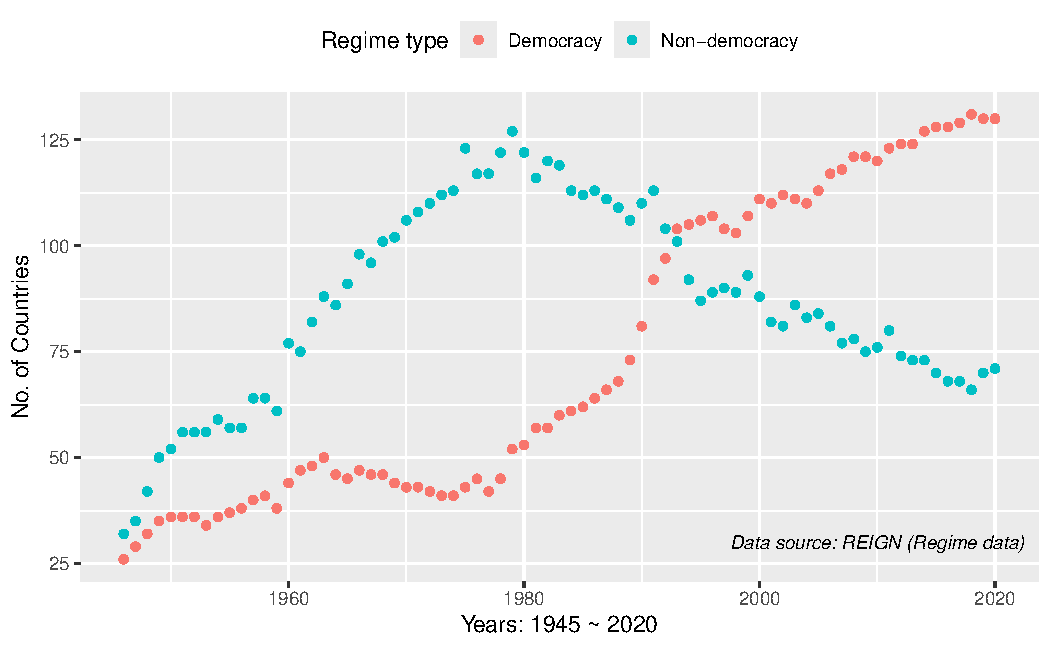
\includegraphics{coups_and_autocoups_files/figure-pdf/fig-democracy-1.pdf}

}

\caption{\label{fig-democracy}Comparison of the number of democratic and
non-democratic countries (1945-2020)}

\end{figure}%

However, a ``democratic recession'' has emerged in recent years
(\citeproc{ref-diamond2008}{Diamond 2008}). Freedom House reports an
18th consecutive year of global freedom decline in 2023
(\citeproc{ref-freedomhouse2024freedom}{Freedom House 2024}). While few
countries have completely regressed to autocracy, the average global
democracy level has fallen back to pre-2000 levels. Notably, democratic
backsliding often occurs within regimes, with democracies becoming less
liberal and autocracies becoming less competitive
(\citeproc{ref-mechkova2017}{Mechkova, Lührmann, and Lindberg 2017}).

This research highlights irregular power transitions as a significant
factor in democratic backsliding within regimes. These transitions,
often coups or autocoups, violate democratic norms and disrupt the path
towards stable democracies. Leaders who gain power through irregular
means often resort to undemocratic tactics to maintain control, creating
a vicious cycle of eroding democratic institutions.

Our findings suggest that the shorter lifespans and potentially severe
consequences associated with coups may deter potential coup leaders.
Conversely, autocoups appear to be a more tempting option for
power-hungry leaders due to their higher success rates, seemingly
moderate consequences, and extended leader tenure after the autocoup.
This trend may explain the decline in classic coups since the 1990s
alongside the rise of autocoups (\citeproc{ref-bermeo2016}{Bermeo
2016}).

\section{Limitations and directions for future
research}\label{limitations-and-directions-for-future-research}

This study offers a novel framework for analysing irregular power
transitions, but some limitations require further exploration:

\begin{itemize}
\item
  \textbf{Data refinement:} Defining and classifying autocoups is a new
  approach. Future research should validate this classification system
  through additional studies and expert evaluations.
\item
  \textbf{Data harmonization:} The current analysis faces challenges due
  to mismatched units (country-year vs.~leader) between coup and
  autocoup datasets. Future efforts should explore data harmonization
  techniques for more robust comparisons.
\item
  \textbf{Democratic backsliding:} While this study establishes a
  connection between irregular power transitions and democratic
  backsliding, further empirical evidence is needed to solidify this
  link.
\end{itemize}

Several avenues exist for future research:

\begin{itemize}
\item
  \textbf{Terminology and data collection:} Refining the ``autocoup''
  concept and achieving wider recognition will facilitate more accurate
  and comprehensive data collection.
\item
  \textbf{Dataset expansion:} Expanding the autocoup dataset with more
  cases and integrating it with data on other irregular leadership
  transitions can provide a more holistic view of political survival
  after these events.
\item
  \textbf{Power dynamics and long-term impacts:} Utilizing this dataset,
  future studies can delve deeper into power dynamics at play and
  explore the long-term consequences of irregular transitions on
  political systems, particularly regarding democratic backsliding,
  breakdown, and personalization of power.
\end{itemize}

In conclusion, this study sheds light on the dynamics of irregular power
transitions, specifically focusing on coups and autocoups. By redefining
autocoups, classifying the dataset, analysing determinants, and
comparing leader longevity, we establish a framework for understanding
irregular transitions and leader survival. This work contributes to a
deeper understanding of democratic resilience and political stability.
Future research can build upon this foundation by conducting further
empirical analyses based on the novel autocoup dataset and continuing to
refine the framework.

\newpage

\chapter*{References}\label{references}
\addcontentsline{toc}{chapter}{References}

\phantomsection\label{refs}
\begin{CSLReferences}{1}{0}
\bibitem[\citeproctext]{ref-aidt2019}
Aidt, Toke, and Gabriel Leon. 2019. {``The Coup.''} Edited by Roger D.
Congleton, Bernard Grofman, and Stefan Voigt, February.
\url{https://doi.org/10.1093/oxfordhb/9780190469771.013.15}.

\bibitem[\citeproctext]{ref-arriagadaherrera1988}
Arriagada Herrera, Genaro. 1988. \emph{Pinochet: the politics of power}.
Thematic studies in Latin America. Boston: Unwin Hyman.

\bibitem[\citeproctext]{ref-baturo2022}
Baturo, Alexander, and Jakob Tolstrup. 2022. {``Incumbent Takeovers.''}
\emph{Journal of Peace Research} 60 (2): 373--86.
\url{https://doi.org/10.1177/00223433221075183}.

\bibitem[\citeproctext]{ref-bermeo2016}
Bermeo, Nancy. 2016. {``On Democratic Backsliding.''} \emph{Journal of
Democracy} 27 (1): 5--19. \url{https://doi.org/10.1353/jod.2016.0012}.

\bibitem[\citeproctext]{ref-cameron1998a}
Cameron, Maxwell A. 1998. {``Latin American Autogolpes : Dangerous
Undertows in the Third Wave of Democratisation.''} \emph{Third World
Quarterly} 19 (2): 219--39.
\url{https://doi.org/10.1080/01436599814433}.

\bibitem[\citeproctext]{ref-chin2021}
Chin, John J, David B Carter, and Joseph G Wright. 2021. {``The
Varieties of Coups D{'}état: Introducing the Colpus Dataset.''}
\emph{International Studies Quarterly} 65 (4): 1040--51.
\url{https://doi.org/10.1093/isq/sqab058}.

\bibitem[\citeproctext]{ref-diamond2008}
Diamond, Larry. 2008. \emph{The Spirit of Democracy: The Struggle to
Build Free Societies Throughout the World}. Macmillan.

\bibitem[\citeproctext]{ref-fariss2022}
Fariss, Christopher J., Therese Anders, Jonathan N. Markowitz, and
Miriam Barnum. 2022. {``New Estimates of Over 500 Years of Historic GDP
and Population Data.''} \emph{Journal of Conflict Resolution} 66 (3):
553--91. \url{https://doi.org/10.1177/00220027211054432}.

\bibitem[\citeproctext]{ref-frantz2016}
Frantz, Erica, and Elizabeth A. Stein. 2016. {``Countering Coups:
Leadership Succession Rules in Dictatorships.''} \emph{Comparative
Political Studies} 50 (7): 935--62.
\url{https://doi.org/10.1177/0010414016655538}.

\bibitem[\citeproctext]{ref-freedomhouse2024freedom}
Freedom House. 2024. {``Freedom in the World 2024.''}
\url{https://freedomhouse.org/sites/default/files/2024-02/FIW_2024_DigitalBooklet.pdf}.

\bibitem[\citeproctext]{ref-gassebner2016}
Gassebner, Martin, Jerg Gutmann, and Stefan Voigt. 2016. {``When to
Expect a Coup d{'}état? An Extreme Bounds Analysis of Coup
Determinants.''} \emph{Public Choice} 169 (3-4): 293--313.
\url{https://doi.org/10.1007/s11127-016-0365-0}.

\bibitem[\citeproctext]{ref-geddes1999}
Geddes, Barbara. 1999. {``What Do We Know About Democratization After
Twenty Years?''} \emph{Annual Review of Political Science} 2 (1):
115--44. \url{https://doi.org/10.1146/annurev.polisci.2.1.115}.

\bibitem[\citeproctext]{ref-geddes2014}
Geddes, Barbara, Joseph Wright, and Erica Frantz. 2014. {``Autocratic
Breakdown and Regime Transitions: A New Data Set.''} \emph{Perspectives
on Politics} 12 (2): 313--31.
\url{https://doi.org/10.1017/s1537592714000851}.

\bibitem[\citeproctext]{ref-ginsburg2019}
Ginsburg, Tom, and Zachary Elkins. 2019. {``One Size Does Not Fit
All.''} In, 37--52. Oxford University Press.
\url{https://doi.org/10.1093/oso/9780198837404.003.0003}.

\bibitem[\citeproctext]{ref-goemans2009}
Goemans, Henk E., Kristian Skrede Gleditsch, and Giacomo Chiozza. 2009.
{``Introducing Archigos: A Dataset of Political Leaders.''}
\emph{Journal of Peace Research} 46 (2): 269--83.
\url{https://doi.org/10.1177/0022343308100719}.

\bibitem[\citeproctext]{ref-huntington1991democratization}
Huntington, Samuel P. 1991. {``The Third Wave: Democratization in the
Late Twentieth Century.''} \emph{Norman, OK: University of Oklahoma}.

\bibitem[\citeproctext]{ref-krishnarajan2019}
Krishnarajan, Suthan. 2019. {``Economic Crisis, Natural Resources, and
Irregular Leader Removal in Autocracies.''} \emph{International Studies
Quarterly} 63 (3): 726--41. \url{https://doi.org/10.1093/isq/sqz006}.

\bibitem[\citeproctext]{ref-leon2013a}
Leon, Gabriel. 2013. {``Loyalty for Sale? Military Spending and Coups
d{'}etat.''} \emph{Public Choice} 159 (3-4): 363--83.
\url{https://doi.org/10.1007/s11127-013-0124-4}.

\bibitem[\citeproctext]{ref-marshall2005current}
Marshall, Monty G. 2005. {``Current Status of the World's Major Episodes
of Political Violence.''} \emph{Report to Political Instability Task
Force.(3 February)}.

\bibitem[\citeproctext]{ref-mechkova2017}
Mechkova, Valeriya, Anna Lührmann, and Staffan I. Lindberg. 2017. {``How
Much Democratic Backsliding?''} \emph{Journal of Democracy} 28 (4):
162--69. \url{https://doi.org/10.1353/jod.2017.0075}.

\bibitem[\citeproctext]{ref-peyton2024}
Peyton, Buddy, Joseph Bajjalieh, Dan Shalmon, Michael Martin, and Emilio
Soto. 2024. {``Cline Center Coup d{'}état Project Dataset.''} University
of Illinois at Urbana-Champaign.
\url{https://doi.org/10.13012/B2IDB-9651987_V7}.

\bibitem[\citeproctext]{ref-powell2012}
Powell, Jonathan. 2012. {``Determinants of the Attempting and Outcome of
Coups d{'}état.''} \emph{Journal of Conflict Resolution} 56 (6):
1017--40. \url{https://doi.org/10.1177/0022002712445732}.

\bibitem[\citeproctext]{ref-powell2011}
Powell, Jonathan M, and Clayton L Thyne. 2011. {``Global Instances of
Coups from 1950 to 2010: A New Dataset.''} \emph{Journal of Peace
Research} 48 (2): 249--59.
\url{https://doi.org/10.1177/0022343310397436}.

\bibitem[\citeproctext]{ref-powell2018}
Powell, Jonathan, Christopher Faulkner, William Dean, and Kyle Romano.
2018. {``Give Them Toys? Military Allocations and Regime Stability in
Transitional Democracies.''} \emph{Democratization} 25 (7): 1153--72.
\url{https://doi.org/10.1080/13510347.2018.1450389}.

\bibitem[\citeproctext]{ref-roessler2011}
Roessler, Philip. 2011. {``The Enemy Within: Personal Rule, Coups, and
Civil War in Africa.''} \emph{World Politics} 63 (2): 300--346.
\url{https://doi.org/10.1017/s0043887111000049}.

\bibitem[\citeproctext]{ref-singh2016}
Singh, Naunihal. 2016. \emph{Seizing Power}. Johns Hopkins University
Press. \url{https://doi.org/10.1353/book.31450}.

\bibitem[\citeproctext]{ref-sudduth2017}
Sudduth, Jun Koga. 2017. {``Strategic Logic of Elite Purges in
Dictatorships.''} \emph{Comparative Political Studies} 50 (13):
1768--1801. \url{https://doi.org/10.1177/0010414016688004}.

\bibitem[\citeproctext]{ref-thyne2019}
Thyne, Clayton L., and Jonathan Powell. 2019. {``Coup Research,''}
October. \url{https://doi.org/10.1093/acrefore/9780190846626.013.369}.

\bibitem[\citeproctext]{ref-wintrobe2019}
Wintrobe, Ronald. 2019. {``Are There Types of Dictatorship?''} Edited by
Roger D. Congleton, Bernard Grofman, and Stefan Voigt, February.
\url{https://doi.org/10.1093/oxfordhb/9780190469771.013.13}.

\end{CSLReferences}



\end{document}
